\documentclass{beamer}
% imprimir
% \documentclass[handout]{beamer} 
% \usepackage{pgfpages}
% \pgfpagesuselayout{4 on 1}[a4paper,landscape,border shrink=5mm]

\mode<presentation> {
  \usetheme{Warsaw}
  \setbeamercovered{transparent}
}

\usebackgroundtemplate{
\includegraphics[width=\paperwidth]{format/libresoft-bg.png}}
\usepackage[spanish]{babel}
\usepackage[utf8]{inputenc}

\usepackage{times}
\usepackage[T1]{fontenc}

%% Metadatos del PDF.
\hypersetup{  
  pdftitle={Virtualización con software libre},
  pdfauthor={Miguel Vidal},
  pdfcreator={GSyC/Libresoft},
  pdfproducer=PDFLaTeX,
  pdfsubject={Virtualización con Qemu},
}
%%


\defbeamertemplate*{footline}{shadow theme}
{%
  \leavevmode%
  \hbox{\begin{beamercolorbox}[wd=.5\paperwidth,ht=2.5ex,dp=1.125ex,leftskip=.3cm plus1fil,rightskip=.3cm]{author in head/foot}%
    \usebeamerfont{author in head/foot}\insertframenumber\,/\,\inserttotalframenumber\hfill
\includegraphics[scale=0.40]{format/cc-by-80x15.png} \hspace{0.1cm}\insertshortauthor 
% \usebeamerfont{author in head/foot} 
\includegraphics[width=0.7cm]{format/cc-by.png} \hfill\insertshortauthor
  \end{beamercolorbox}%
  \begin{beamercolorbox}[wd=.5\paperwidth,ht=2.5ex,dp=1.125ex,leftskip=.3cm,rightskip=.3cm plus1fil]{title in head/foot}%
    \usebeamerfont{title in head/foot}\insertshorttitle%
  \end{beamercolorbox}}%
  \vskip0pt%
}

\begin{document}

\title{El arte de virtualizar}
\subtitle{Virtualización con Qemu}
\author{Miguel Vidal \and José Castro}
\institute{\{mvidal,jfcastro\}@libresoft.es} 
\date[CASUL 2011]{Curso de Arquitectura de Servidores, 2011}

\frame{
\maketitle
\begin{center}

\includegraphics[width=6cm]{format/gsyc-urjc}
\end{center}
}

%% License slide
\begin{frame}
  \vspace{2cm}
  \begin{flushright}
    {\small (cc) 2011 Miguel Vidal, Jose Castro.} \\
%    \vspace{0.25cm}
    \medskip
    {\scriptsize Esta presentación se distribuye bajo \\ licencia Creative Commons Reconocimiento 3.0 España}
%    \vspace{0.10cm}
  \end{flushright}
  \begin{center}
    \href{http://creativecommons.org/licenses/by/3.0/es}{
\includegraphics[width=2cm]{format/cc-by.png}} \\
    {\tiny \url{http://creativecommons.org/licenses/by/3.0/es}}
  \end{center}
\end{frame}%%


\usebackgroundtemplate{}

% \AtBeginSubsection[]
% {
%  \begin{frame}<beamer>{Índice}
%    \tableofcontents[currentsection,currentsubsection]
%  \end{frame}
% }


%%%%%%%%%%%%%%%%%%%%%%%%%%%%%%%%%%%%%%%%%%%%%%%%%%%%%%%%%%%%%%%%%%%%%%%
% \section{Virtualización con Qemu}
%%%%%%%%%%%%%%%%%%%%%%%%%%%%%%%%%%%%%%%%%%%%%%%%%%%%%%%%%%%%%%%%%%%%%%%

\begin{frame}
\frametitle{¿Qué es Qemu?}

\begin{definition}
Emulador de procesadores mediante traducción dinámica de binarios.
\end{definition}

\begin{itemize}
\item Puede ejecutar código compilado en una CPU en otra CPU (\alert{emulación}). 
\item Convierte el código binario de la arquitectura fuente en código comprensible para la arquitectura huésped.
\item Puede también comportarse como una VMM para \alert{virtualizar} \textit{guests} sin modificar dentro de una misma arquitectura.
\end{itemize}

\end{frame}

\begin{frame}
\frametitle{Virtualización con Qemu}

\begin{itemize}
\item Dispone de un modo acelerado (KQEMU o KVM/Linux) para x86.
\item Soporta como invitados a  Linux, Solaris, Microsoft Windows, DOS y BSD.
\item Emula las arquitecturas hardware x86, x86-64 (AMD64/Intel64), ARM, Alpha, ETRAX CRIS, MIPS, MicroBlaze, PowerPC y SPARC. 
\end{itemize}

\end{frame}

%%%%%%%%%%%%%%%%%%%%%%%%%%%%%%%%%%%%%%%%%%%%%%%%%%%%%%%%%%%%%%%%%%%%%%%

\begin{frame}
\frametitle{Emulación con Qemu}

\begin{center}
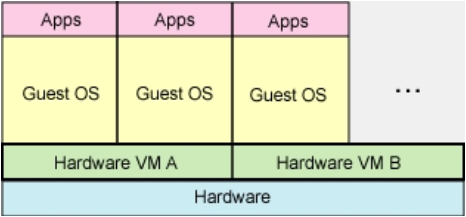
\includegraphics[width=6cm,clip=false]{figs/emulation.png}
\end{center}

\end{frame}


%%%%%%%%%%%%%%%%%%%%%%%%%%%%%%%%%%%%%%%%%%%%%%%%%%%%%%%%%%%%%%%%%%%%%%%

\begin{frame}
\frametitle{Qemu: Crear imagen para el FS}

\small
Crear imagen que alojará el sistema de ficheros:
\begin{semiverbatim}
\alert{\$ qemu-img create -f qcow2 disk1.img 2G}

Formatting 'disk1.img', fmt=qcow2 size=2147483648 

encryption=off cluster\_size=0 
\end{semiverbatim}

\medskip
Comprobamos que la expansión es dinámica (qcow2):
\begin{semiverbatim}
\alert{\$ ls -lh disk1.img} 
 
-rw-r--r--  1 mvidal  users   193K May 27 11:48 disk1.img
\end{semiverbatim}

\end{frame}

%%%%%%%%%%%%%%%%%%%%%%%%%%%%%%%%%%%%%%%%%%%%%%%%%%%%%%%%%%%%%%%%%%%%%%%

\begin{frame}[fragile]
\frametitle{Qemu: Formato qcow2}

\begin{itemize}
\item Formato de imagen de disco avanzado de Qemu y KVM. 
\item Soporta Copy-on-write: la imagen solo tiene los cambios hechos sobre una imagen de solo-lectura. 
\item Soporta snapshots.
\item Cifrado AES y compresión zlib opcionales.
\end{itemize}

\end{frame}


%%%%%%%%%%%%%%%%%%%%%%%%%%%%%%%%%%%%%%%%%%%%%%%%%%%%%%%%%%%%%%%%%%%%%%%

\begin{frame}
\frametitle{Qemu: Instalar el SO}

Instalar un Sistema Operativo con 256MB de RAM:
\begin{semiverbatim}
\$ qemu -hda openbsd.img -cdrom install49.iso \\ 

\hspace{4mm} -m 256 -net nic -boot d
\end{semiverbatim}

Instalar un SO (Debian) emulando la arquitectura Sparc:

\begin{semiverbatim}
\$ qemu-system-sparc64 -m 256 -monitor stdio \\ 

\hspace{4mm} -hda virtual.img \\

\hspace{4mm} -cdrom debian-6.0.1a-sparc-netinst.iso -boot d
\end{semiverbatim}
\end{frame}

%%%%%%%%%%%%%%%%%%%%%%%%%%%%%%%%%%%%%%%%%%%%%%%%%%%%%%%%%%%%%%%%%%%%%%%

\begin{frame}
% \frametitle{Emulación de arquitectura Sparc}

\begin{figure}
  \centering
	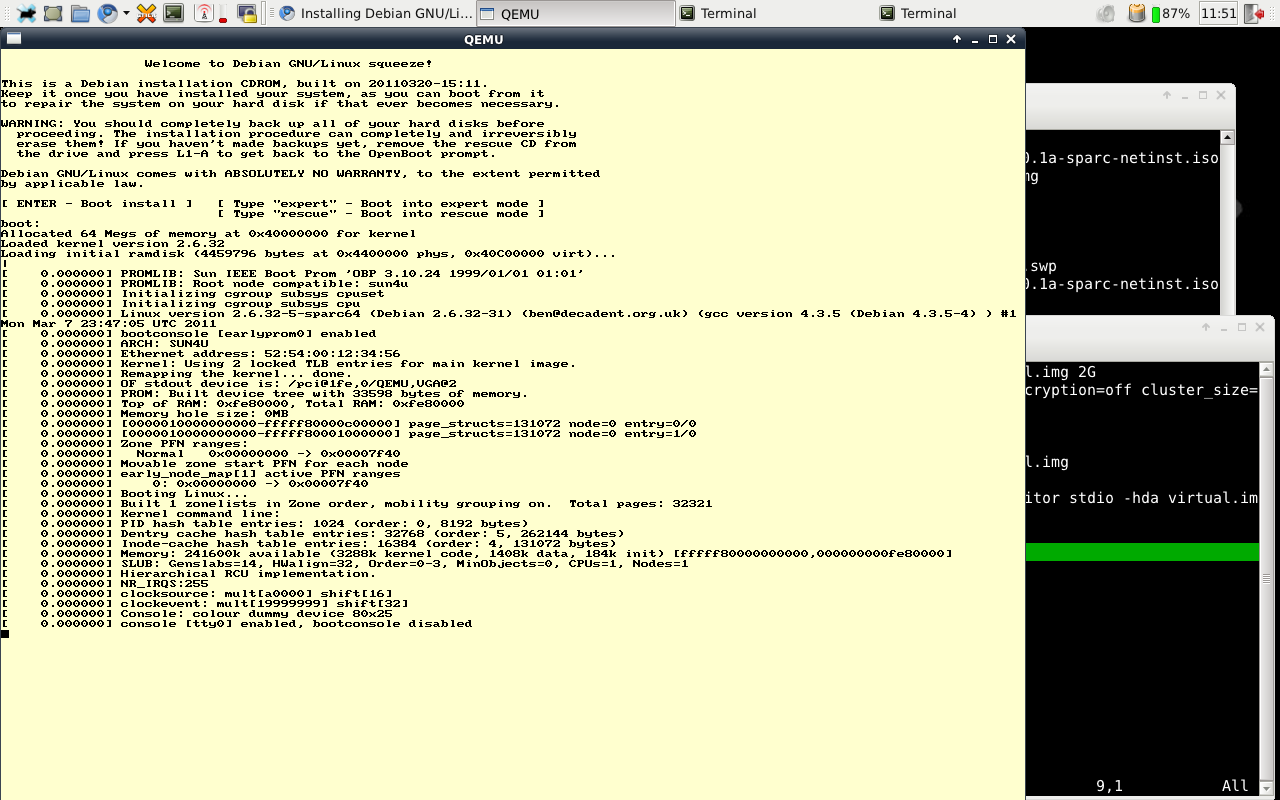
\includegraphics[width=11cm,clip=false]{figs/qemu-sparc-install.png}
  \caption{\scriptsize{Emulación de una arquitectura Sparc (Debian) desde x86 (OpenBSD)}}
%  \label{fig:ejemplo}
\end{figure}

\end{frame}



%%%%%%%%%%%%%%%%%%%%%%%%%%%%%%%%%%%%%%%%%%%%%%%%%%%%%%%%%%%%%%%%%%%%%%%

\begin{frame}
\frametitle{Qemu: arrancar el SO}

Arrancar normalmente el Sistema Operativo virtualizado:
\begin{semiverbatim}
qemu -hda debian.img -m 256
\end{semiverbatim}

Arrancar una VM (OpenBSD) pasando opciones complejas de red mediante script:
\begin{semiverbatim}
\small
\$ qemu-system-x86\_64 -net nic,vlan=0 -net tap,vlan=0\\

\hspace{10mm} -net nic -net tap, \alert{script=/etc/qemu-ifup} \\ 

\hspace{10mm} -no-fd-bootchk -hda OpenBSD.img

\end{semiverbatim}
\end{frame}

\begin{frame}
\frametitle{Ejemplo de script de arranque para red}

Script de arranque para configurar la red con un dispositivo virtual:
\begin{semiverbatim}
\$ cat /etc/qemu-ifup

\#! /bin/sh

\medskip

\# Set the tun device into layer2 mode

ifconfig \$1 10.0.0.10 netmask 255.255.255.0 link0 

\end{semiverbatim}
\end{frame}

%%%%%%%%%%%%%%%%%%%%%%%%%%%%%%%%%%%%%%%%%%%%%%%%%%%%%%%%%%%%%%%%%%%%%%%


\end{document}

